\documentclass[12pt,a4paper]{article}

\usepackage[utf8]{inputenc}
\usepackage[T1]{fontenc}
\usepackage[brazil]{babel}
\usepackage{amsmath,amssymb}
\usepackage{graphicx}
\usepackage{hyperref}
\usepackage{booktabs}
\usepackage{geometry}
\usepackage{float}
\usepackage{caption}
\usepackage{subcaption}
\usepackage{algorithm}
\usepackage{algpseudocode}
\usepackage{xcolor}
\usepackage{array}

\geometry{margin=2.5cm}

\hypersetup{
    colorlinks=true,
    linkcolor=blue,
    urlcolor=blue,
    citecolor=blue
}

\title{\textbf{Redes de Colaboração Musical:\\Análise Estrutural e Diversidade de Gêneros}\\[0.5em]
\large MC859 -- Teoria em Grafos}
\author{Cirilo Morais Frota \\ \texttt{cirilomoraisf@gmail.com}}
\date{Junho de 2026}

\begin{document}

\maketitle

\begin{abstract}
Este trabalho modela colaborações entre os 100 artistas mais ouvidos do Spotify como um grafo não-direcionado ponderado, no qual vértices representam artistas e arestas representam co-créditos em faixas. O grafo resultante possui 6.874 vértices e 26.955 arestas. A análise principal investiga se artistas com colaborações mais diversas em termos de gênero musical exibem maior popularidade. Para cada artista-semente, calcula-se a entropia de Shannon sobre os gêneros dos vizinhos (metrica de diversidade $H$) e compara-se com \emph{monthly listeners} do Spotify, betweenness centrality e gênero principal. Os testes estatísticos (correlação de Spearman, Mann-Whitney U e regressão OLS) indicam que $H$ não prediz popularidade de forma estatisticamente significativa ($\rho = +0{,}096$, $p = 0{,}365$), mas correlaciona-se significativamente com centralidade de intermediação ($\rho = +0{,}315$, $p = 0{,}002$). O repositório público com a implementação e as instâncias está disponível em \url{https://github.com/cmmmf/MC859-Teoria-em-Grafos}.
\end{abstract}

\tableofcontents
\newpage

% ─────────────────────────────────────────────────────────────────
\section{Introdução}
% ─────────────────────────────────────────────────────────────────

Colaborações entre artistas de diferentes gêneros musicais são fenômenos frequentes na indústria fonográfica moderna. Do ponto de vista de redes complexas, essa dinâmica pode ser modelada como um grafo de colaboração, no qual a estrutura topológica revela padrões sobre como artistas se conectam e influenciam uns aos outros.

Este projeto propõe modelar essas interações como um grafo não-direcionado ponderado, onde:
\begin{itemize}
    \item \textbf{Vértices} representam artistas musicais;
    \item \textbf{Arestas} representam colaborações (co-crédito em uma faixa);
    \item \textbf{Peso} de uma aresta é o número de faixas em que dois artistas colaboraram;
    \item \textbf{Atributos} de vértice incluem nome, gênero musical principal e contagem de faixas.
\end{itemize}

Os objetivos específicos são: (i) coletar dados de artistas e colaborações via APIs públicas; (ii) construir um grafo de colaboração com atributos de gênero; (iii) extrair métricas estruturais da rede; e (iv) analisar, com rigor estatístico, a relação entre diversidade de gênero nas colaborações e popularidade dos artistas.

O repositório público com a implementação completa e as instâncias em formato GraphML está em:
\begin{center}
    \url{https://github.com/cmmmf/MC859-Teoria-em-Grafos}
\end{center}

% ─────────────────────────────────────────────────────────────────
\section{Coleta de Dados}
% ─────────────────────────────────────────────────────────────────

\subsection{Fontes de dados}

Utilizaram-se duas APIs públicas complementares:

\begin{enumerate}
    \item \textbf{Spotify Web API} (via biblioteca \texttt{spotipy}): utilizada para obter os 100 artistas com mais \emph{monthly listeners} globais e o catálogo de faixas de cada um. Para cada faixa, extraímos os IDs de todos os artistas creditados.

    \item \textbf{MusicBrainz API}: utilizada para obter o gênero musical principal de cada artista. O MusicBrainz mantém metadados colaborativos (gêneros e \emph{tags} com contagem de votos), o que permite selecionar o gênero mais representativo de cada artista. A taxa de requisições foi limitada a 1 req/s conforme os termos de uso da API.
\end{enumerate}

\subsection{Pipeline de extração}

O pipeline foi implementado em Python 3.14 e consiste nas seguintes etapas:

\begin{enumerate}
    \item \textbf{Seleção dos artistas-semente}: lista manual dos 100 artistas com mais ouvintes mensais no Spotify (coletada em maio/junho de 2026), armazenada em \texttt{internal/data/top100artists.py} com nome, ID Spotify e monthly listeners.

    \item \textbf{Coleta de faixas}: para cada artista-semente, o módulo \texttt{track\_fetcher.py} consulta a Spotify Web API e extrai todas as faixas do álbum discográfico. Cada linha do arquivo \texttt{tracks.csv} armazena o ID da faixa, nome, IDs de todos os artistas creditados e nomes correspondentes.

    \item \textbf{Coleta de gêneros}: o módulo \texttt{graph\_builder.py} e o script \texttt{enrich\_neighbor\_genres.py} consultam o MusicBrainz para obter o gênero principal de cada artista (seeds e vizinhos com peso $\geq 2$). Os resultados são cacheados incrementalmente em \texttt{artist\_genres.csv}, tornando o processo resiliente a interrupções.
\end{enumerate}

\subsection{Volume de dados}

O arquivo \texttt{tracks.csv} contém as faixas discográficas dos 100 artistas-semente. O grafo resultante possui 6.874 artistas únicos e 26.955 pares de colaboração distintos. O arquivo \texttt{artist\_genres.csv} contém os gêneros principais de todos os artistas para os quais o MusicBrainz retornou dados.

% ─────────────────────────────────────────────────────────────────
\section{Criação das Instâncias}
% ─────────────────────────────────────────────────────────────────

\subsection{Construção do grafo}

O grafo de colaboração foi construído pelo módulo \texttt{CollaborationGraphBuilder} em \texttt{graph\_builder.py}. Para cada faixa em \texttt{tracks.csv}, todos os pares de artistas co-creditados recebem uma aresta (ou incremento de peso se a aresta já existir). Artistas sem colaborações recebem um vértice isolado.

O grafo é salvo no formato \textbf{GraphML} (\texttt{collab\_graph.graphml}), disponível no repositório. Cada vértice armazena os atributos: \texttt{name}, \texttt{main\_genre}, \texttt{total\_tracks} e \texttt{degree}. Cada aresta armazena o atributo \texttt{weight}.

\subsection{Métricas estruturais}

A Tabela~\ref{tab:metricas} resume as métricas básicas do grafo.

\begin{table}[H]
\centering
\caption{Métricas estruturais do grafo de colaboração.}
\label{tab:metricas}
\begin{tabular}{lr}
\toprule
\textbf{Métrica} & \textbf{Valor} \\
\midrule
Número de vértices $|V|$ & 6.874 \\
Número de arestas $|E|$ & 26.955 \\
Grau médio $\bar{k} = 2|E|/|V|$ & 7,8426 \\
Número de componentes conexas & 5 \\
\bottomrule
\end{tabular}
\end{table}

\subsection{Distribuição de graus}

A Figura~\ref{fig:graus} mostra a distribuição dos graus dos vértices. A distribuição é fortemente assimétrica à direita (\emph{heavy-tailed}), padrão típico de redes de colaboração: a maioria dos artistas possui poucos parceiros, enquanto alguns hubs altamente conectados (e.g., Snoop Dogg com grau 1.252, Future com 438) concentram a maior parte das conexões.

\begin{figure}[H]
    \centering
    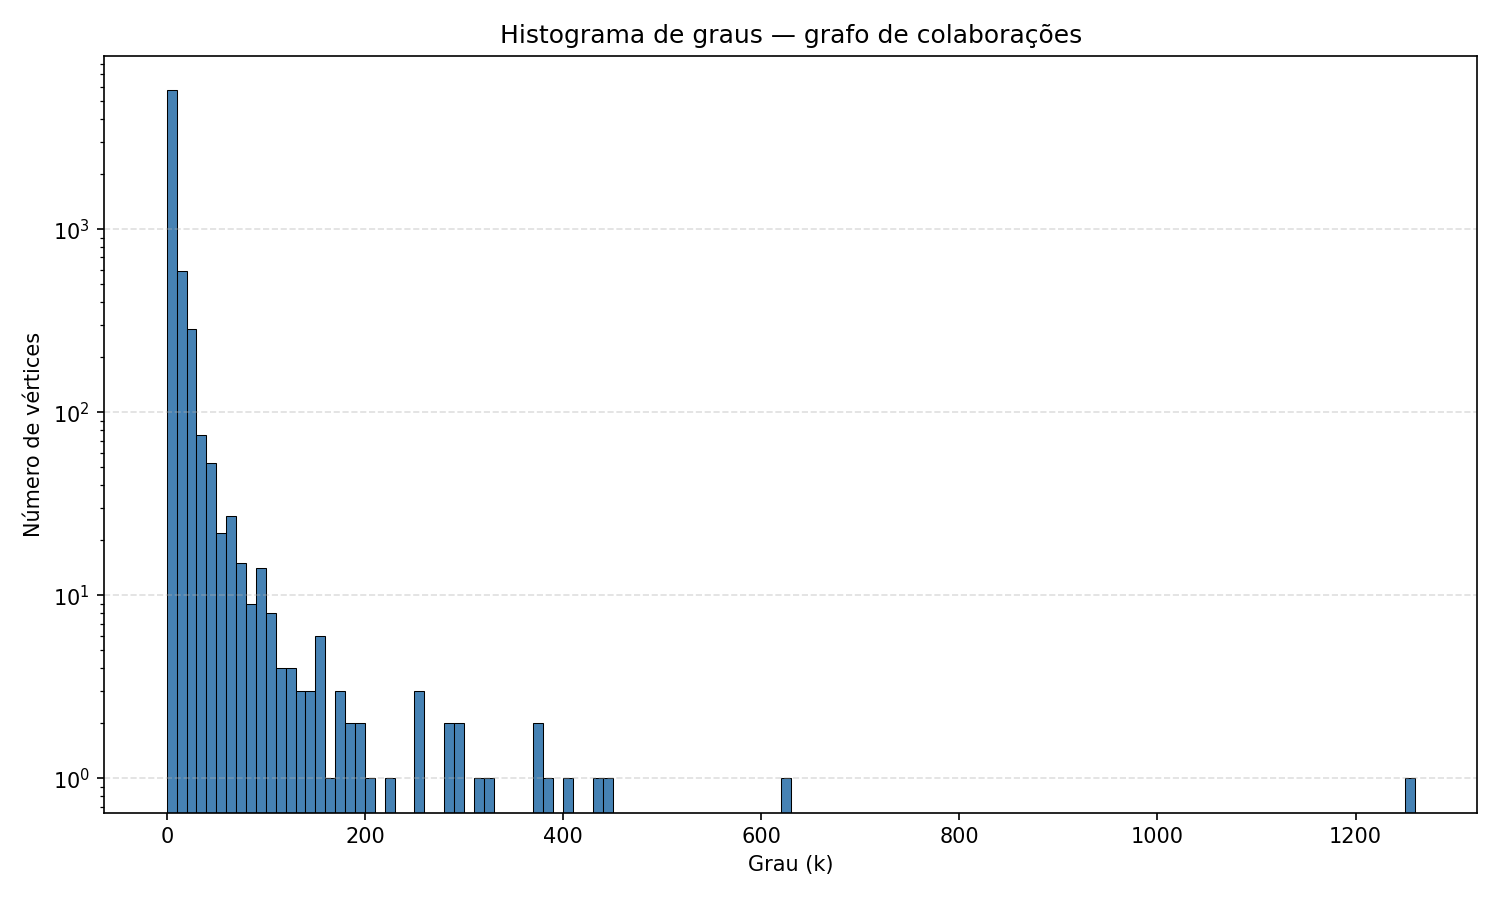
\includegraphics[width=0.75\textwidth]{degree_distribution.png}
    \caption{Distribuição dos graus dos vértices do grafo de colaboração.}
    \label{fig:graus}
\end{figure}

\subsection{Componentes conexas}

O grafo possui 5 componentes conexas. A componente gigante contém 6.864 vértices (99,85\% do total), indicando que praticamente toda a rede é alcançável. As demais componentes são pequenas e isoladas, conforme a Tabela~\ref{tab:componentes}.

\begin{table}[H]
\centering
\caption{Tamanho das componentes conexas.}
\label{tab:componentes}
\begin{tabular}{cc}
\toprule
\textbf{Tamanho (vértices)} & \textbf{Número de componentes} \\
\midrule
6.864 & 1 \\
4     & 1 \\
3     & 1 \\
2     & 1 \\
1     & 1 \\
\bottomrule
\end{tabular}
\end{table}

As componentes menores correspondem a artistas cujos colaboradores não estão conectados à componente gigante: por exemplo, \textit{Kanye West Tribute Band} (isolado), \textit{Imperial Age} e \textit{Infinitas} (par), \textit{Cigarettes After Sex}, \textit{Goody Grace} e \textit{Lexi Jayde} (trio), e o quarteto \textit{Black Sabbath}, \textit{Keith Moon}, \textit{Led Zeppelin}, \textit{The Strokes}.

A Figura~\ref{fig:componentes} ilustra a distribuição dos tamanhos das componentes.

\begin{figure}[H]
    \centering
    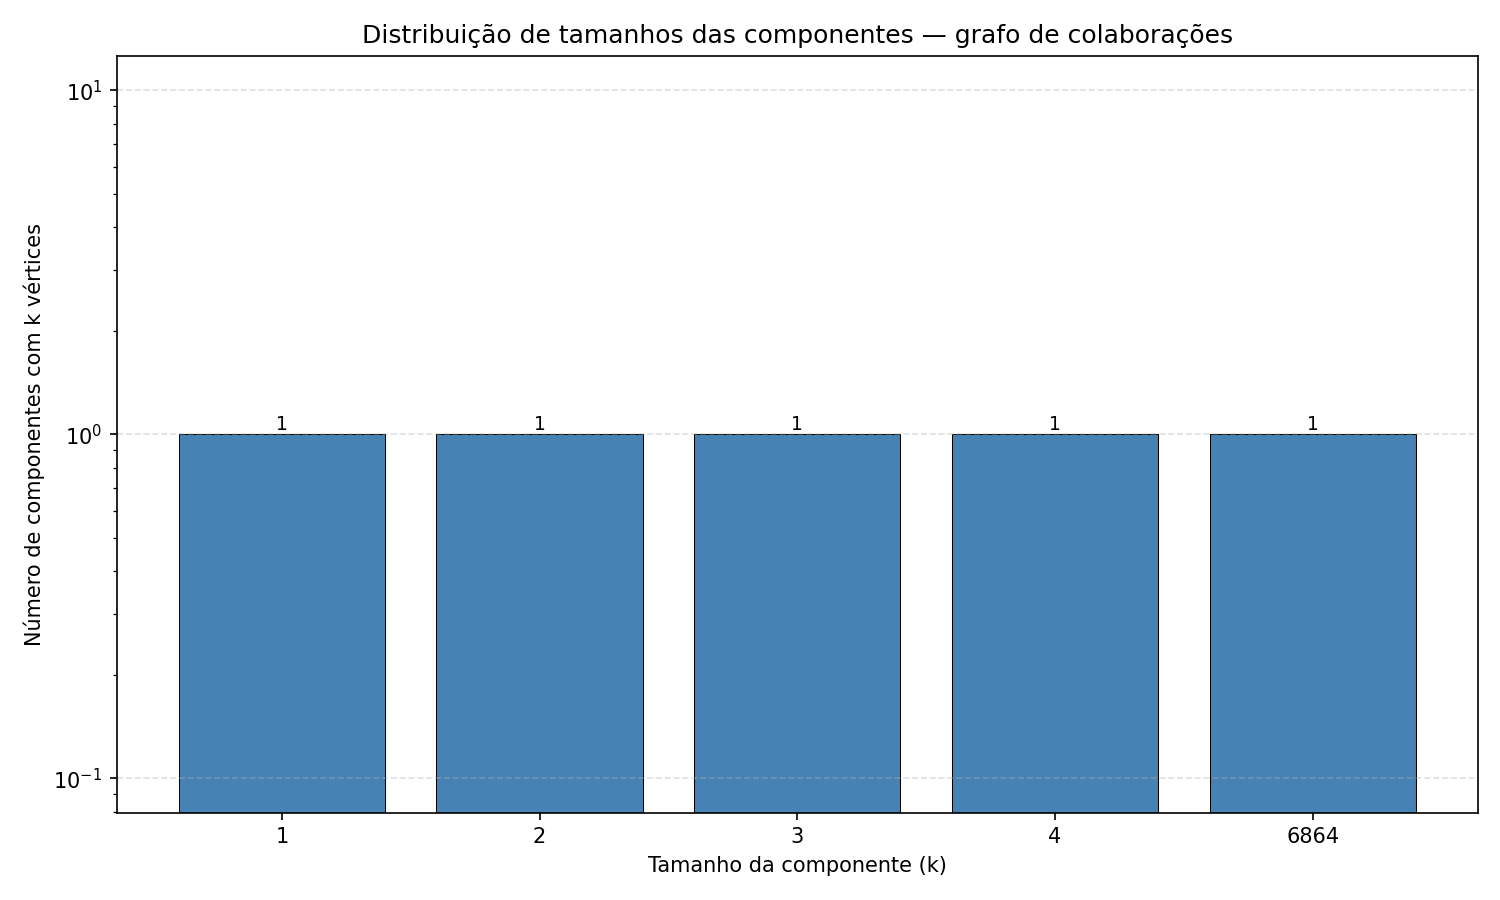
\includegraphics[width=0.65\textwidth]{component_sizes.png}
    \caption{Distribuição dos tamanhos das componentes conexas.}
    \label{fig:componentes}
\end{figure}

% ─────────────────────────────────────────────────────────────────
\section{Algoritmos e Métodos}
% ─────────────────────────────────────────────────────────────────

\subsection{Entropia de Shannon como medida de diversidade}

Para cada artista-semente $v$, define-se a diversidade de colaborações como a entropia de Shannon sobre os gêneros dos vizinhos, ponderada pelo número de colaborações:

\begin{equation}
    H(v) = -\sum_{g \in G_v} \frac{w_g}{W_v} \log_2 \frac{w_g}{W_v}
    \label{eq:shannon}
\end{equation}

onde $G_v$ é o conjunto de gêneros dos vizinhos de $v$ (com peso de aresta $\geq 2$), $w_g$ é a soma dos pesos das arestas para vizinhos de gênero $g$, e $W_v = \sum_g w_g$. Vizinhos sem gênero identificado são excluídos. Um valor $H = 0$ indica que todas as colaborações são com artistas de um único gênero; valores altos indicam diversidade entre muitos gêneros.

\begin{algorithm}[H]
\caption{Cálculo da entropia de Shannon para um vértice $v$}
\begin{algorithmic}[1]
\Require grafo $G$, vértice $v$, limiar de peso \textit{min\_weight}
\Ensure entropia $H(v)$ ou \textbf{None} se sem vizinhos válidos
\State $\text{genre\_weight} \gets \{\}$
\For{cada vizinho $u$ de $v$ com $\text{peso}(v,u) \geq \text{min\_weight}$}
    \State $g \gets \text{gênero}(u)$
    \If{$g \neq \emptyset$}
        \State $\text{genre\_weight}[g] \mathrel{+}= \text{peso}(v, u)$
    \EndIf
\EndFor
\State $W \gets \sum_g \text{genre\_weight}[g]$
\If{$W = 0$} \Return \textbf{None} \EndIf
\Return $-\sum_g \dfrac{\text{genre\_weight}[g]}{W} \cdot \log_2\!\left(\dfrac{\text{genre\_weight}[g]}{W}\right)$
\end{algorithmic}
\end{algorithm}

\subsection{Betweenness centrality (Brandes)}

A centralidade de intermediação (\emph{betweenness centrality}) normalizada de um vértice $v$ é:

\begin{equation}
    C_B(v) = \frac{1}{(n-1)(n-2)} \sum_{s \neq v \neq t} \frac{\sigma_{st}(v)}{\sigma_{st}}
\end{equation}

onde $\sigma_{st}$ é o número de caminhos mínimos entre $s$ e $t$, e $\sigma_{st}(v)$ é o número desses caminhos que passam por $v$. O algoritmo de Brandes~\cite{brandes2001} computa essa métrica em $O(|V| \cdot |E|)$, utilizado via NetworkX.

\subsection{Testes estatísticos}

\subsubsection*{Correlação de Spearman}

Dado que as distribuições de $H$, popularidade e betweenness não são normais, utilizou-se o coeficiente de correlação de Spearman $\rho$, que é baseado em postos e não faz suposições sobre a distribuição subjacente.

\subsubsection*{Teste de Mann-Whitney U}

Para comparar diretamente os grupos de baixa e alta diversidade, aplicou-se o teste de Mann-Whitney U (equivalente não-paramétrico do teste $t$ de Student para amostras independentes) entre os artistas do quartil inferior ($Q_1$) e superior ($Q_3$) de $H$. O tamanho de efeito foi quantificado pela correlação biserial de postos:

\begin{equation}
    r = 1 - \frac{2U}{n_1 \cdot n_2}
\end{equation}

onde $U$ é a estatística do teste e $n_1$, $n_2$ são os tamanhos dos grupos.

\subsubsection*{Regressão OLS}

Ajustou-se um modelo de regressão linear por mínimos quadrados ordinários (OLS):

\begin{equation}
    \log_{10}(\text{listeners}) = \beta_0 + \beta_1 H + \beta_2 C_B + \sum_g \gamma_g \cdot \mathbf{1}[\text{gênero} = g] + \varepsilon
\end{equation}

O uso de $\log_{10}(\text{listeners})$ como variável dependente lineariza a relação com a popularidade, cuja distribuição é fortemente assimétrica. A inclusão de dummies de gênero controla para o efeito confundidor do gênero musical.

% ─────────────────────────────────────────────────────────────────
\section{Resultados}
% ─────────────────────────────────────────────────────────────────

\subsection{Perfil de diversidade dos artistas-semente}

Dos 98 artistas-semente encontrados no grafo, 91 possuem vizinhos com gênero identificado e peso $\geq 2$, permitindo o cálculo de $H$. Os 7 restantes possuem vizinhos insuficientes (somente colaborações de peso 1 ou sem gênero).

A Figura~\ref{fig:distribuicoes} apresenta as distribuições de $H$, popularidade e betweenness. A entropia varia de $0$ (colaborações exclusivamente dentro do mesmo gênero) a $4{,}11$ bits (Elton John, com colaboradores de 17 gêneros distintos).

\begin{figure}[H]
    \centering
    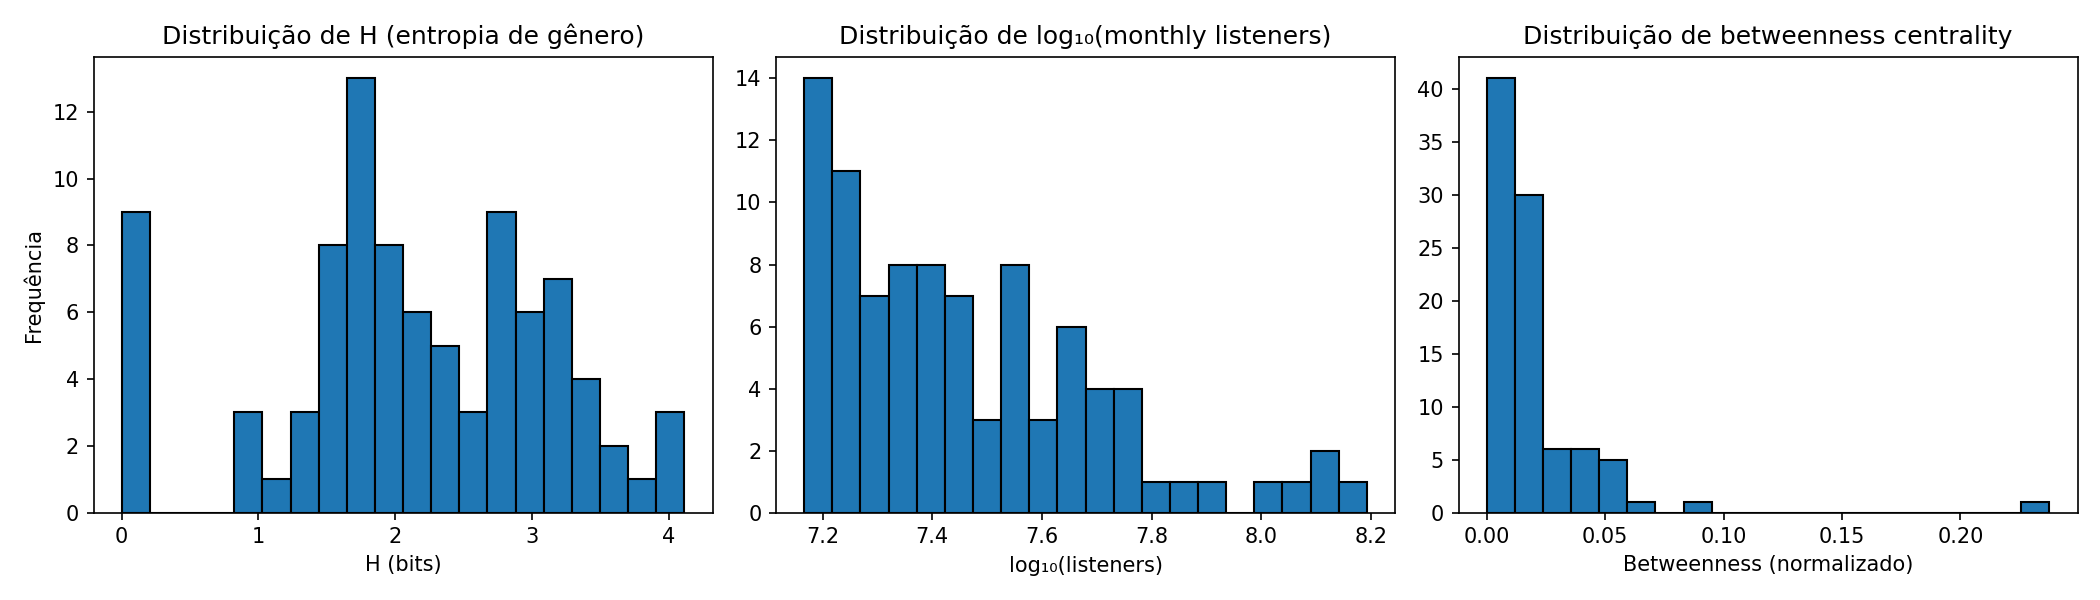
\includegraphics[width=\textwidth]{analysis_distributions.png}
    \caption{Distribuições de entropia de diversidade $H$, log\textsubscript{10}(monthly listeners) e betweenness centrality normalizado.}
    \label{fig:distribuicoes}
\end{figure}

\subsubsection*{Artistas mais diversos}

\begin{table}[H]
\centering
\caption{Artistas com maior entropia de diversidade $H$.}
\label{tab:mais_diversos}
\begin{tabular}{lcc}
\toprule
\textbf{Artista} & \textbf{$H$ (bits)} & \textbf{Gênero principal} \\
\midrule
Elton John         & 4,11 & pop \\
Gorillaz           & 4,02 & alternative rock \\
Calvin Harris      & 3,93 & dance-pop \\
Marshmello         & 3,83 & EDM \\
Charlie Puth       & 3,57 & --- \\
Becky G            & 3,50 & latin \\
Taylor Swift       & 3,46 & pop \\
Coldplay           & 3,45 & alternative rock \\
Meghan Trainor     & 3,42 & doo-wop \\
The Chainsmokers   & 3,33 & electro house \\
\bottomrule
\end{tabular}
\end{table}

\subsubsection*{Artistas menos diversos ($H = 0$)}

Os artistas com $H = 0$ possuem todos os seus colaboradores frequentes do mesmo gênero: The Rolling Stones, Metallica, The Beatles, One Direction, Arctic Monkeys, Red Hot Chili Peppers, Pink Floyd, The Neighbourhood e Led Zeppelin. Todos são bandas de rock clássico ou pop, refletindo a homogeneidade de gênero nesses nichos.

\subsection{Correlações de Spearman}

\begin{table}[H]
\centering
\caption{Correlações de Spearman entre diversidade, popularidade e centralidade.}
\label{tab:spearman}
\begin{tabular}{lcc}
\toprule
\textbf{Par} & $\rho$ & $p$\textbf{-valor} \\
\midrule
$H$ vs.\ $\log_{10}(\text{listeners})$ & $+0{,}096$ & $0{,}365$ \\
betweenness vs.\ $\log_{10}(\text{listeners})$ & $-0{,}006$ & $0{,}952$ \\
$H$ vs.\ betweenness & $+0{,}315$ & $0{,}002$ \\
\bottomrule
\end{tabular}
\end{table}

Apenas a correlação entre $H$ e betweenness é estatisticamente significativa. Diversidade de colaborações e centralidade de intermediação não se traduzem em maior popularidade medida por ouvintes mensais.

\subsection{Comparação entre grupos: Mann-Whitney U}

Comparou-se o $\log_{10}(\text{listeners})$ entre os artistas do quartil inferior ($H \leq 1{,}618$, $n=23$) e superior ($H \geq 2{,}881$, $n=23$) de diversidade.

\begin{table}[H]
\centering
\caption{Resultado do teste de Mann-Whitney U.}
\label{tab:mwu}
\begin{tabular}{lc}
\toprule
\textbf{Estatística} & \textbf{Valor} \\
\midrule
$U$ & 217,0 \\
$p$-valor (bicaudal) & 0,302 \\
Rank-biserial $r$ & $+0{,}180$ \\
\midrule
Mediana $\log_{10}(\text{listeners})$ -- baixo-$H$ & 7,37 \\
Mediana $\log_{10}(\text{listeners})$ -- alto-$H$  & 7,43 \\
\bottomrule
\end{tabular}
\end{table}

O teste não rejeita a hipótese nula ($p = 0{,}302 > 0{,}05$). O tamanho de efeito é pequeno ($r = +0{,}18$, numa escala de $-1$ a $+1$). A Figura~\ref{fig:boxplot} ilustra graficamente a ausência de diferença relevante entre os grupos.

\begin{figure}[H]
    \centering
    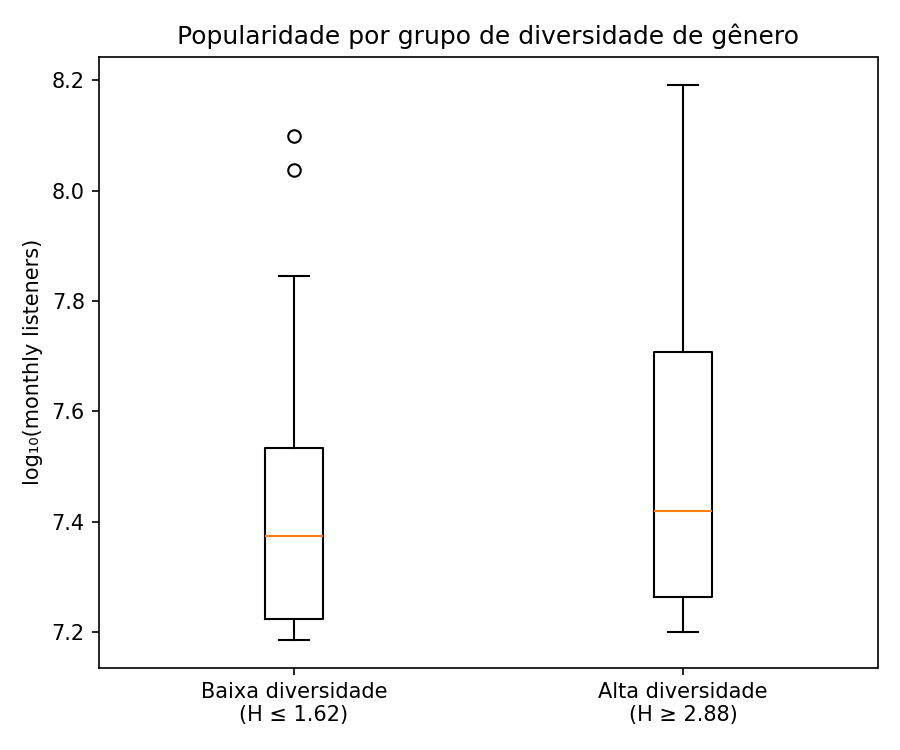
\includegraphics[width=0.55\textwidth]{analysis_boxplot_quartiles.png}
    \caption{Distribuição de popularidade por grupo de diversidade (quartil inferior vs.\ superior de $H$).}
    \label{fig:boxplot}
\end{figure}

\subsection{Regressão OLS}

O modelo OLS com $H$, betweenness e dummies de gênero explica $R^2 = 0{,}215$ da variância em $\log_{10}(\text{listeners})$. Os coeficientes principais são apresentados na Tabela~\ref{tab:ols}.

\begin{table}[H]
\centering
\caption{Coeficientes do modelo OLS (variável dependente: $\log_{10}$(monthly listeners)).}
\label{tab:ols}
\begin{tabular}{lrrrr}
\toprule
\textbf{Variável} & \textbf{Coef.} & \textbf{EP} & $t$ & $p$ \\
\midrule
Intercepto   & $7{,}5915$ & $0{,}2147$ & $35{,}36$ & $< 0{,}001$ \\
$H$          & $-0{,}0198$ & $0{,}0339$ & $-0{,}59$ & $0{,}560$ \\
Betweenness  & $-0{,}7418$ & $1{,}0376$ & $-0{,}71$ & $0{,}477$ \\
\bottomrule
\multicolumn{5}{l}{\footnotesize $n = 91$, $k = 21$ (inclui 18 dummies de gênero), $R^2 = 0{,}215$}
\end{tabular}
\end{table}

Nenhuma variável individual é estatisticamente significativa ao nível de 5\%. O $R^2$ moderado é explicado principalmente pela variabilidade intrínseca entre gêneros, e não por $H$ ou betweenness.

\subsection{Diversidade vs. centralidade}

O scatter plot da Figura~\ref{fig:h_vs_betweenness} mostra a única correlação estatisticamente significativa encontrada: artistas com colaborações mais diversas tendem a ocupar posições mais centrais na rede (betweenness mais alto, $\rho = +0{,}315$, $p = 0{,}002$).

\begin{figure}[H]
    \centering
    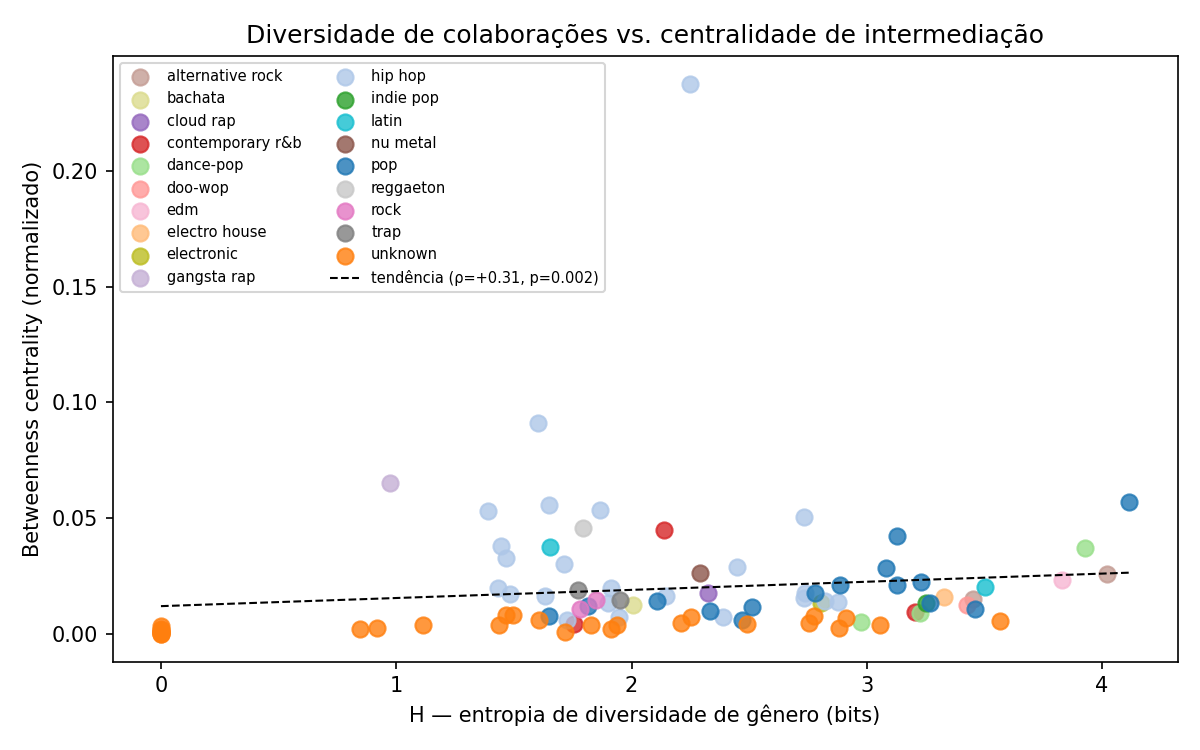
\includegraphics[width=0.75\textwidth]{analysis_h_vs_betweenness.png}
    \caption{Diversidade de colaborações ($H$) vs.\ betweenness centrality por gênero principal.}
    \label{fig:h_vs_betweenness}
\end{figure}

\begin{figure}[H]
    \centering
    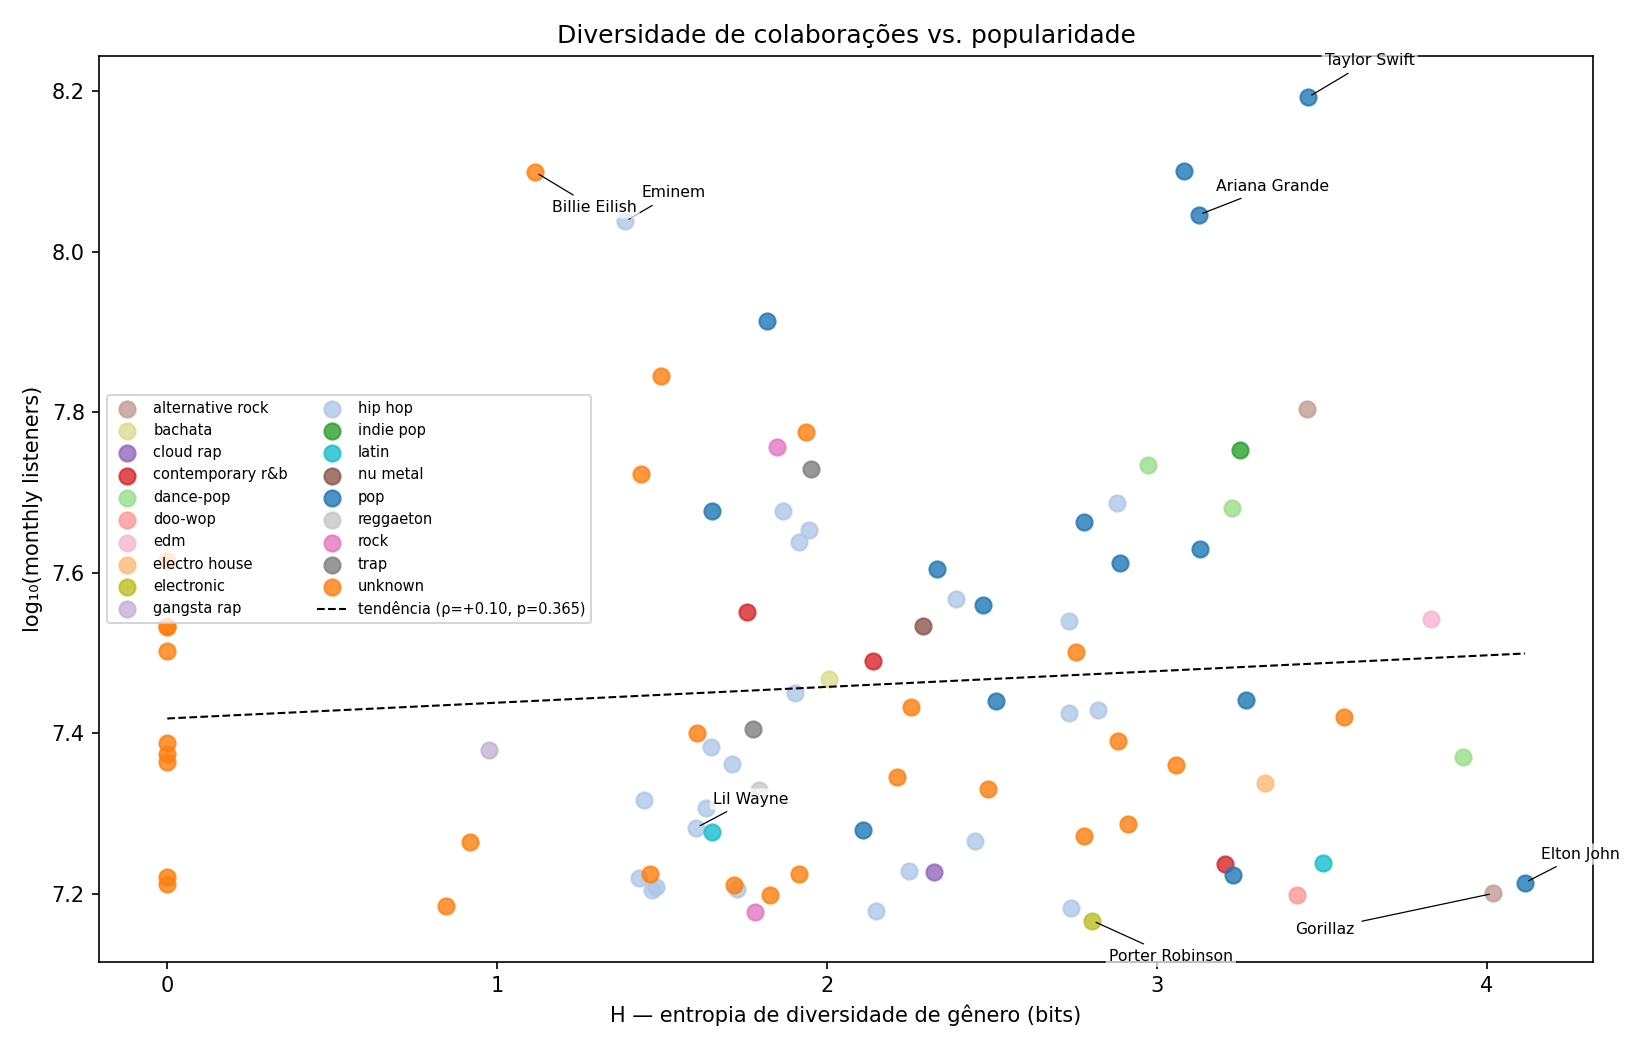
\includegraphics[width=0.75\textwidth]{analysis_h_vs_popularity.png}
    \caption{Diversidade de colaborações ($H$) vs.\ $\log_{10}$(monthly listeners) por gênero principal.}
    \label{fig:h_vs_popularidade}
\end{figure}

% ─────────────────────────────────────────────────────────────────
\section{Análise e Interpretação}
% ─────────────────────────────────────────────────────────────────

\subsection{Diversidade não prediz popularidade}

O conjunto de evidências aponta consistentemente que a diversidade de gênero nas colaborações não aumenta a popularidade dos artistas medida em ouvintes mensais. Isso se mantém em três abordagens complementares: a correlação de Spearman ($\rho = +0{,}096$, $p = 0{,}365$) não é significativa; o teste de Mann-Whitney U ($p = 0{,}302$) não detecta diferença entre os extremos da distribuição de $H$; e a regressão OLS controla para gênero e betweenness e ainda assim não encontra efeito de $H$ ($\beta = -0{,}020$, $p = 0{,}560$).

O tamanho de efeito da comparação Mann-Whitney ($r = +0{,}18$) é pequeno segundo as convenções de Cohen, e com $n = 23$ por grupo o estudo possui poder estatístico limitado para detectar efeitos muito pequenos. Porém, mesmo se o efeito existisse, sua magnitude seria praticamente irrelevante: uma diferença de $0{,}180$ em escala de rank-biserial corresponderia a diferenças de popularidade desprezíveis na escala logarítmica.

\subsection{Diversidade prediz centralidade estrutural}

O achado mais relevante do ponto de vista de redes é a correlação positiva e significativa entre $H$ e betweenness centrality ($\rho = +0{,}315$, $p = 0{,}002$). Artistas que colaboram com parceiros de gêneros variados tendem a atuar como pontes entre diferentes comunidades musicais na rede, acumulando maior centralidade de intermediação.

Isso é interpretável estruturalmente: ao colaborar com artistas de gêneros distintos, um artista cria atalhos entre sub-redes antes desconectadas, aumentando sua participação nos caminhos mínimos da rede global. Exemplos ilustrativos são Elton John (H = 4,11, betweenness = 0,057), Calvin Harris (H = 3,93, betweenness = 0,037) e Gorillaz (H = 4,02, betweenness = 0,026) — todos com alta diversidade e alta centralidade.

\subsection{Popularidade como variável independente}

O resultado nulo para popularidade sugere que os ouvintes mensais são determinados por fatores externos ao grafo de colaboração: qualidade artística, investimento em marketing, acessibilidade do gênero, longevidade de carreira e viralidade em plataformas de streaming. A estrutura de colaborações per se não garante maior audiência, apenas maior posição estrutural na rede.

Vale notar que os artistas analisados já pertencem ao grupo dos 100 mais ouvidos globalmente, o que implica seleção de viés: todos têm popularidade elevada, reduzindo a variância disponível para detectar efeitos. Um estudo com escopo mais amplo poderia encontrar resultados distintos.

\subsection{Padrões por gênero}

Artistas com $H = 0$ pertencem majoritariamente ao rock clássico (The Beatles, Led Zeppelin, Pink Floyd, Metallica, Red Hot Chili Peppers), um gênero historicamente mais fechado a colaborações externas. Em contrapartida, artistas de EDM, dance-pop e latin (Calvin Harris, Marshmello, Becky G) apresentam os maiores valores de $H$, refletindo a tradição desses gêneros de agregar colaboradores de nichos variados.

% ─────────────────────────────────────────────────────────────────
\section{Cronograma}
% ─────────────────────────────────────────────────────────────────

\begin{table}[H]
\centering
\caption{Cronograma de execução do projeto.}
\label{tab:cronograma}
\begin{tabular}{lll}
\toprule
\textbf{Período} & \textbf{Atividade} & \textbf{Status} \\
\midrule
Abr.\ 2026 & Definição do tema e levantamento de APIs & Concluído \\
Abr./Mai.\ 2026 & Coleta de faixas via Spotify API & Concluído \\
Mai.\ 2026 & Construção do grafo e entrega parcial & Concluído \\
Mai./Jun.\ 2026 & Enriquecimento com gêneros (MusicBrainz) & Concluído \\
Jun.\ 2026 & Análise estatística e visualizações & Concluído \\
Jun.\ 2026 & Escrita do relatório final & Concluído \\
\bottomrule
\end{tabular}
\end{table}

% ─────────────────────────────────────────────────────────────────
\section{Conclusão}
% ─────────────────────────────────────────────────────────────────

Este trabalho construiu e analisou um grafo de colaborações musicais com 6.874 artistas e 26.955 arestas, a partir de dados do Spotify e MusicBrainz. A rede é dominada por uma componente gigante contendo 99,85\% dos vértices, com distribuição de graus assimétrica característica de redes complexas reais.

A análise estatística principal investigou se artistas com colaborações mais diversas em gênero são mais populares. Os resultados indicam que não existe associação estatisticamente significativa entre diversidade de colaborações ($H$) e popularidade ($\log_{10}$ de ouvintes mensais), com $p > 0{,}3$ em todos os testes realizados e tamanho de efeito pequeno.

Por outro lado, identificou-se uma correlação positiva e significativa entre diversidade e betweenness centrality ($\rho = +0{,}315$, $p = 0{,}002$): artistas que atravessam fronteiras de gênero em suas colaborações ocupam posições estruturalmente privilegiadas na rede, atuando como pontes entre comunidades musicais distintas.

O código-fonte completo, as instâncias em GraphML e este relatório estão disponíveis em \url{https://github.com/cmmmf/MC859-Teoria-em-Grafos}.

% ─────────────────────────────────────────────────────────────────
\begin{thebibliography}{9}

\bibitem{brandes2001}
U. Brandes,
``A faster algorithm for betweenness centrality,''
\textit{Journal of Mathematical Sociology}, vol.~25, no.~2, pp.~163--177, 2001.

\bibitem{newman2010}
M. E. J. Newman,
\textit{Networks: An Introduction}.
Oxford University Press, 2010.

\bibitem{shannon1948}
C. E. Shannon,
``A mathematical theory of communication,''
\textit{Bell System Technical Journal}, vol.~27, pp.~379--423, 1948.

\bibitem{spotify}
Spotify AB,
``Spotify Web API Reference,''
\url{https://developer.spotify.com/documentation/web-api/}, 2024.

\bibitem{musicbrainz}
MetaBrainz Foundation,
``MusicBrainz API,''
\url{https://musicbrainz.org/doc/MusicBrainz_API}, 2024.

\end{thebibliography}

\end{document}
